\section{Results}
\label{sec:results}
Here we present the results that show the fidelity of the proxy apps compared to their respective parents.
We use several similarity algorithms and compare and contrast the results.  

\subsection{Similarity Matrix Comparison}
\label{sec:SimCom}
%this is in single column
% \begin{figure}[htbp]
% \centering
% 	\begin{minipage}[t]{0.5\textwidth}
% 	\centering
% 	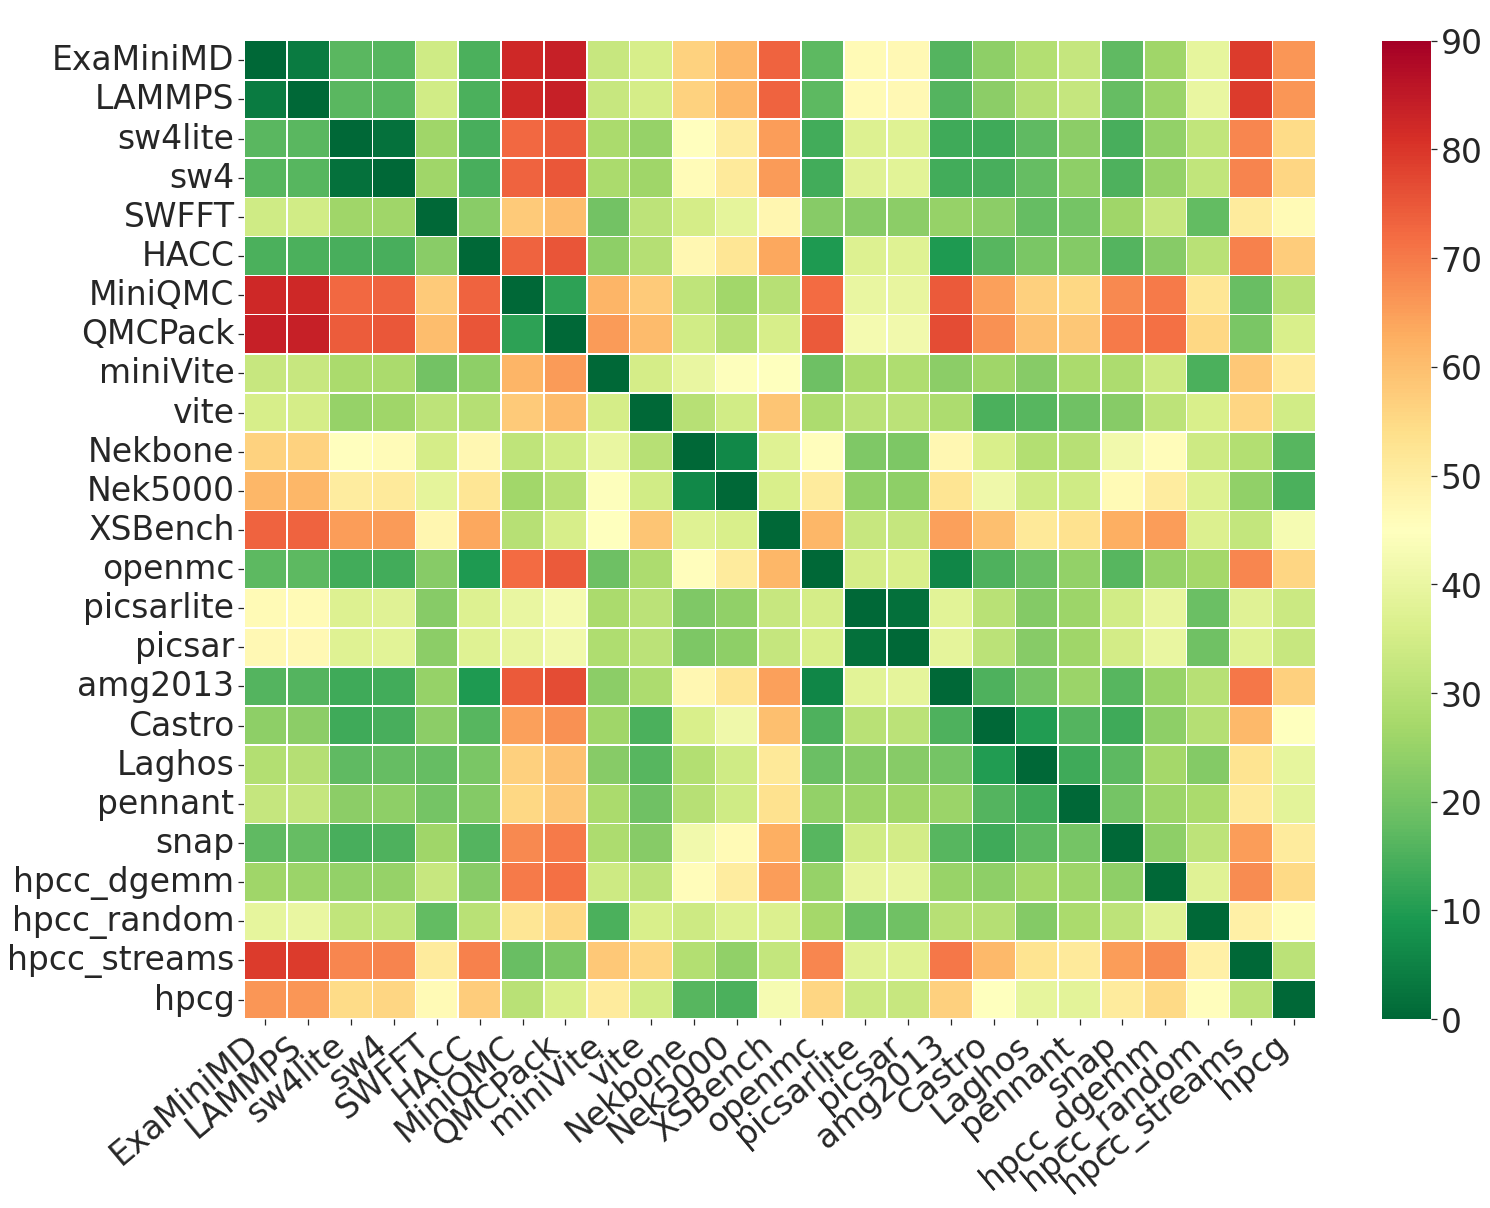
\includegraphics[width=3in]{figs/Cosine_origin_color_nonumber.png}
% 	\vspace*{-5mm}
% 	\caption{Cosine Similarity}
% 	\label{figs:Cosine}
% 	\end{minipage}
% \hspace{.1in}
% \begin{minipage}[t]{0.5\textwidth}
% 	\centering
% 	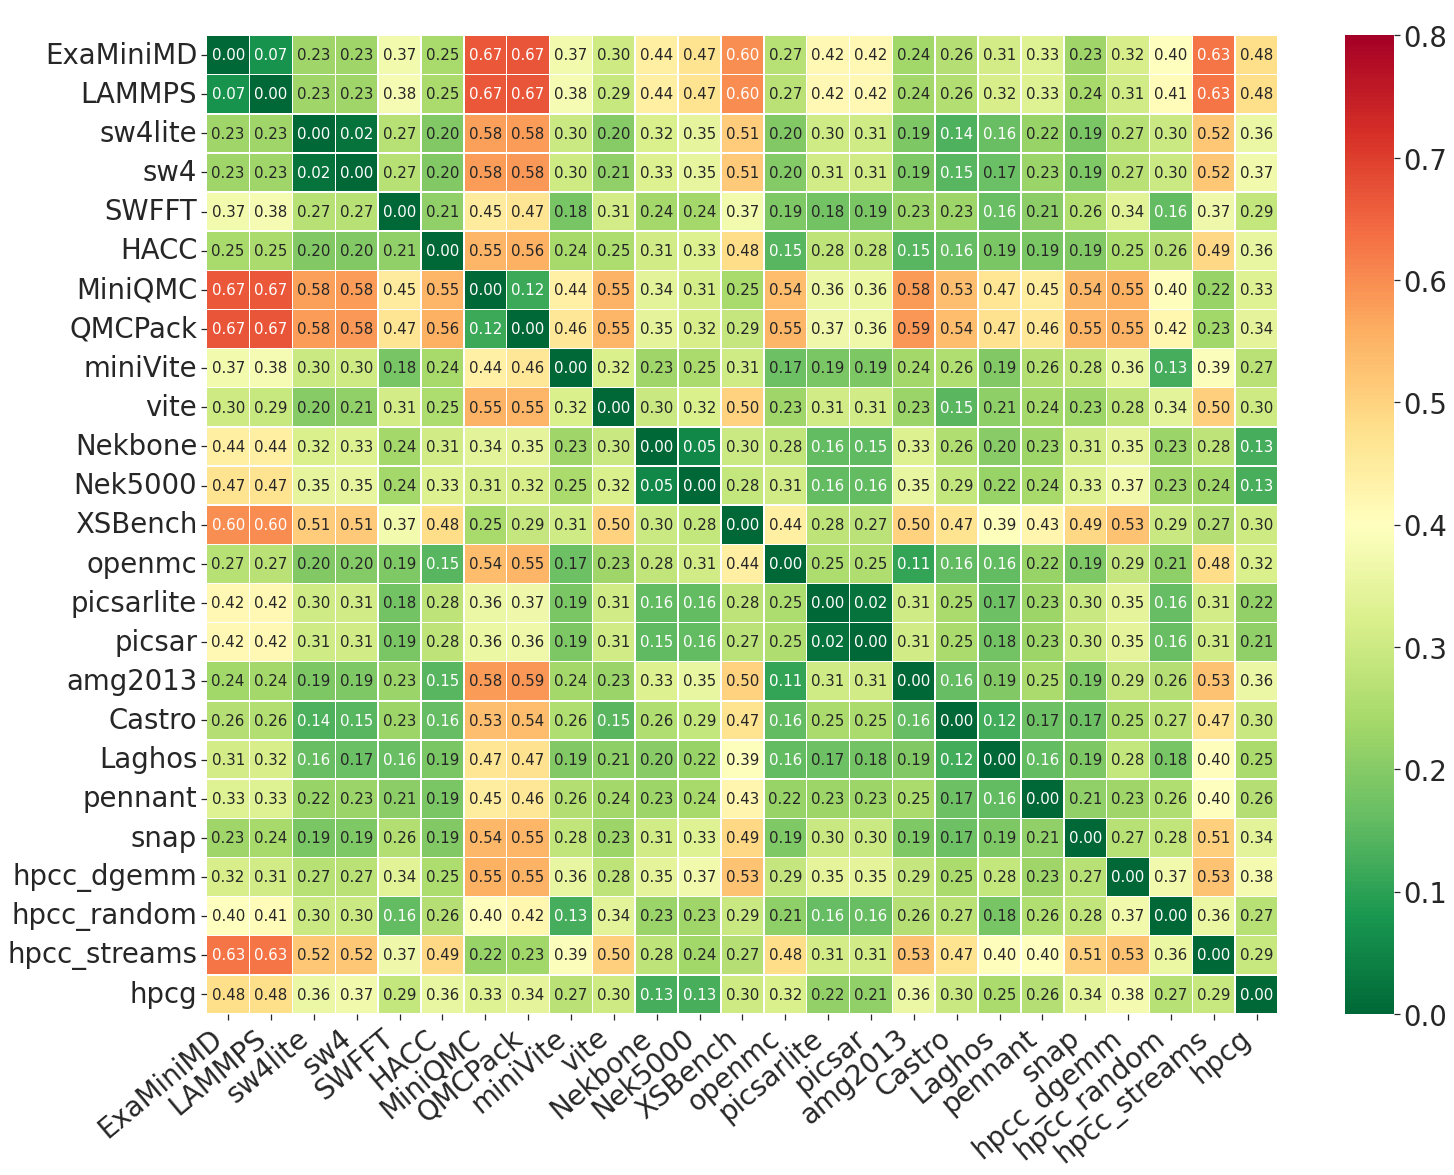
\includegraphics[width=3in]{figs/JS-divergence.png}
% 	\vspace*{-5mm}
% 	\caption{JS divergence}
% 	\label{figs:JS}
% 	\end{minipage}
% \hspace{.1in}
% \begin{minipage}[t]{0.5\textwidth}
% 	\centering
% 	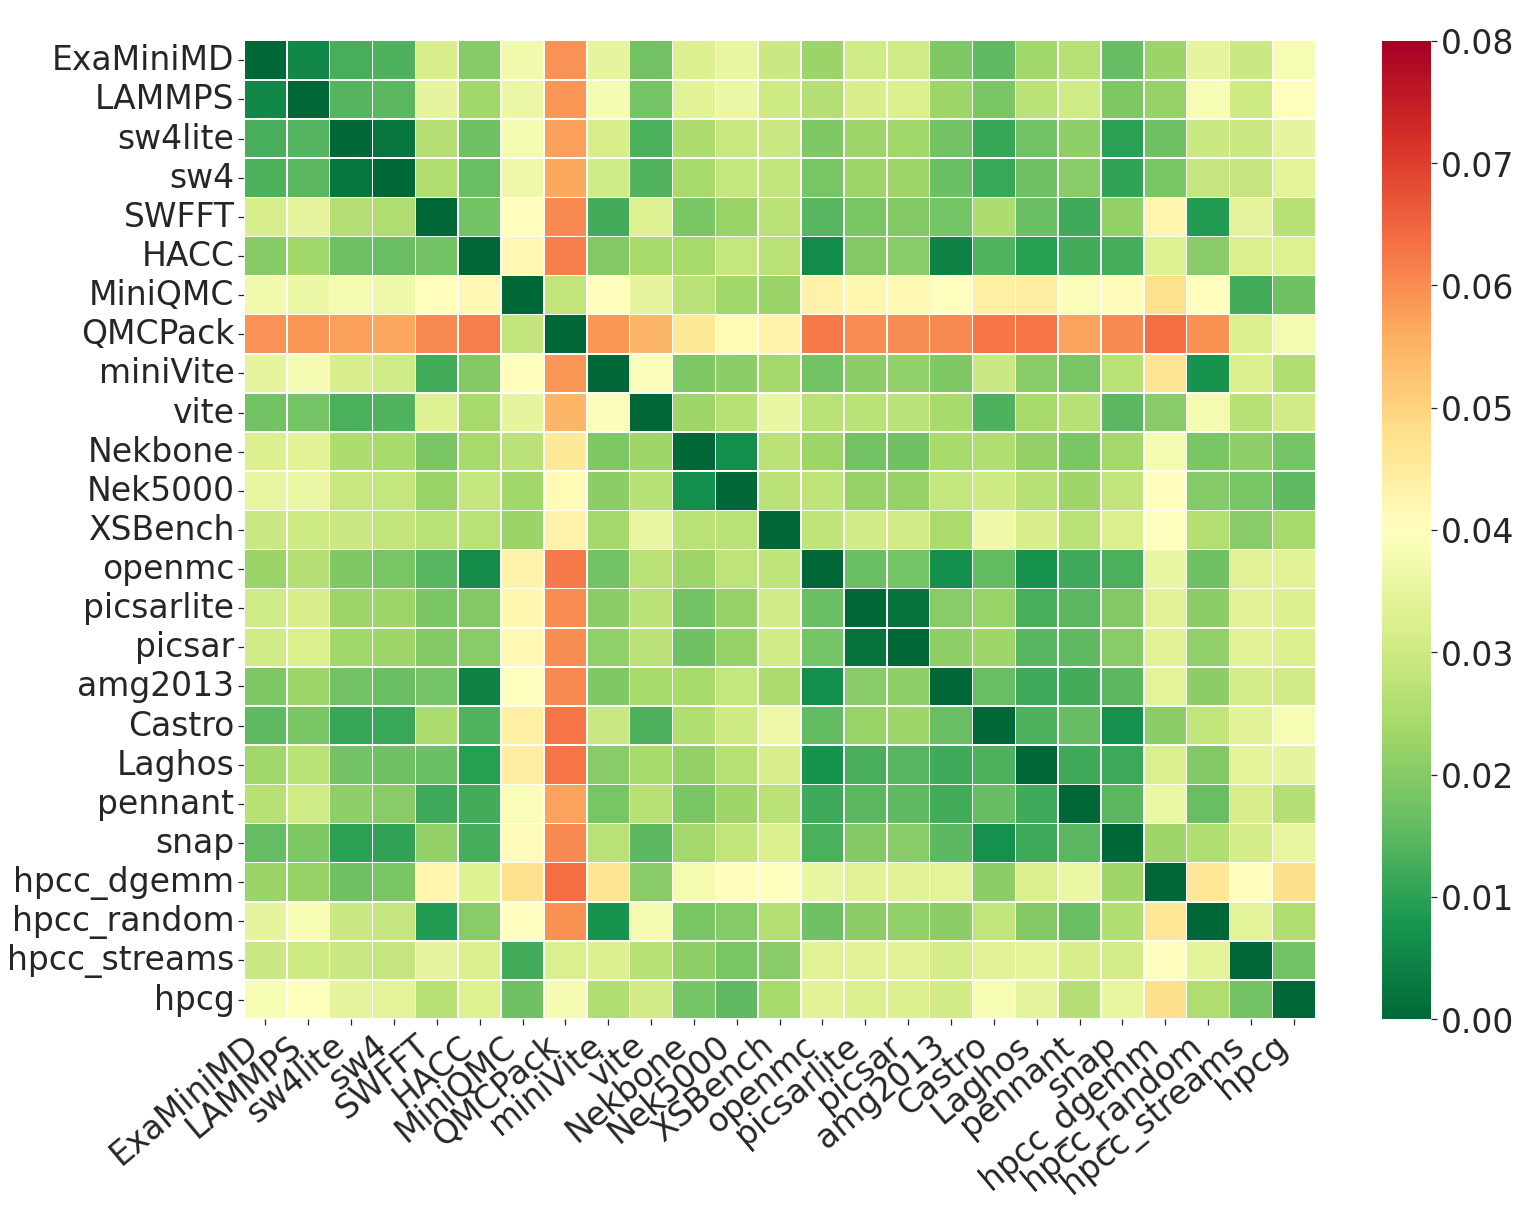
\includegraphics[width=3in]{figs/Wasserstein distance.png}
% 	\vspace*{-5mm}
% 	\caption{Wasserstein distance}
% 	\label{figs:Wasserstein}
% 	\end{minipage}
% \hspace{.1in}	
% \begin{minipage}[t]{0.5\textwidth}
% 	\centering
% 	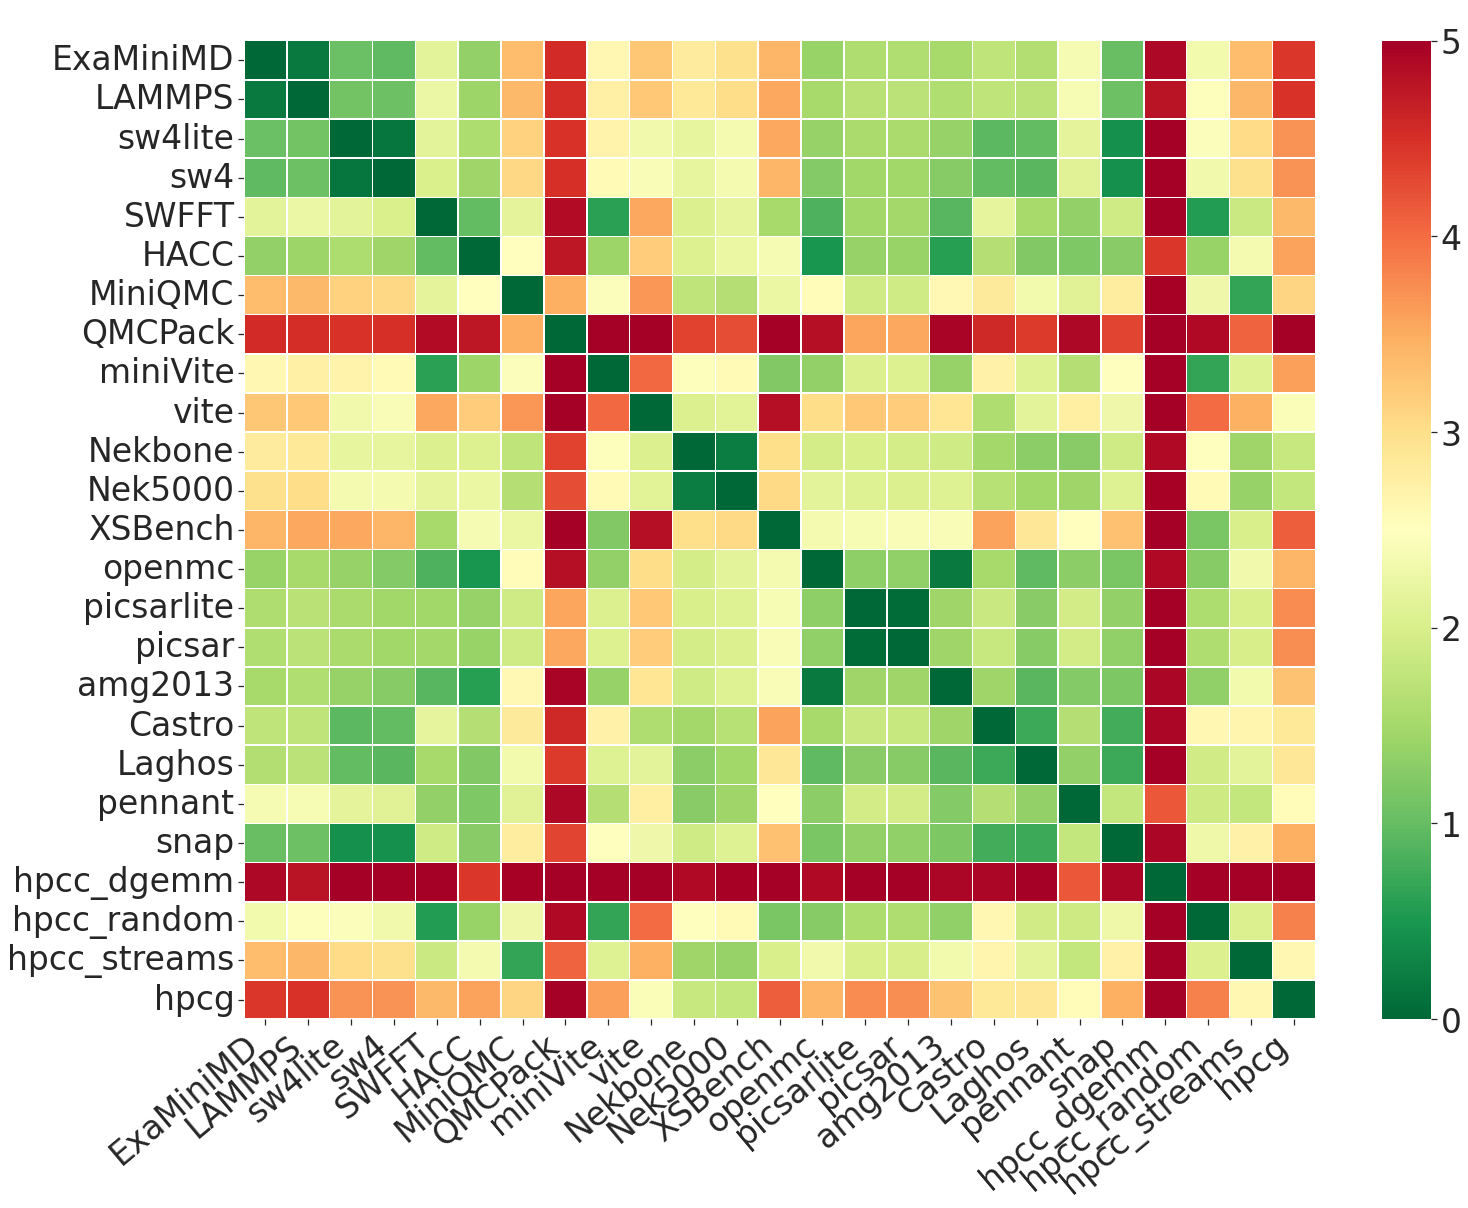
\includegraphics[width=3in]{figs/Mahalanobis distance.png}
% 	\vspace*{-5mm}
% 	\caption{Mahalanobis distance}
% 	\label{figs:Mahalanobis}
% 	\end{minipage}	
% \end{figure}

\begin{figure*}[htbp]
\centering
	\begin{minipage}[t]{0.48\textwidth}
	\centering
	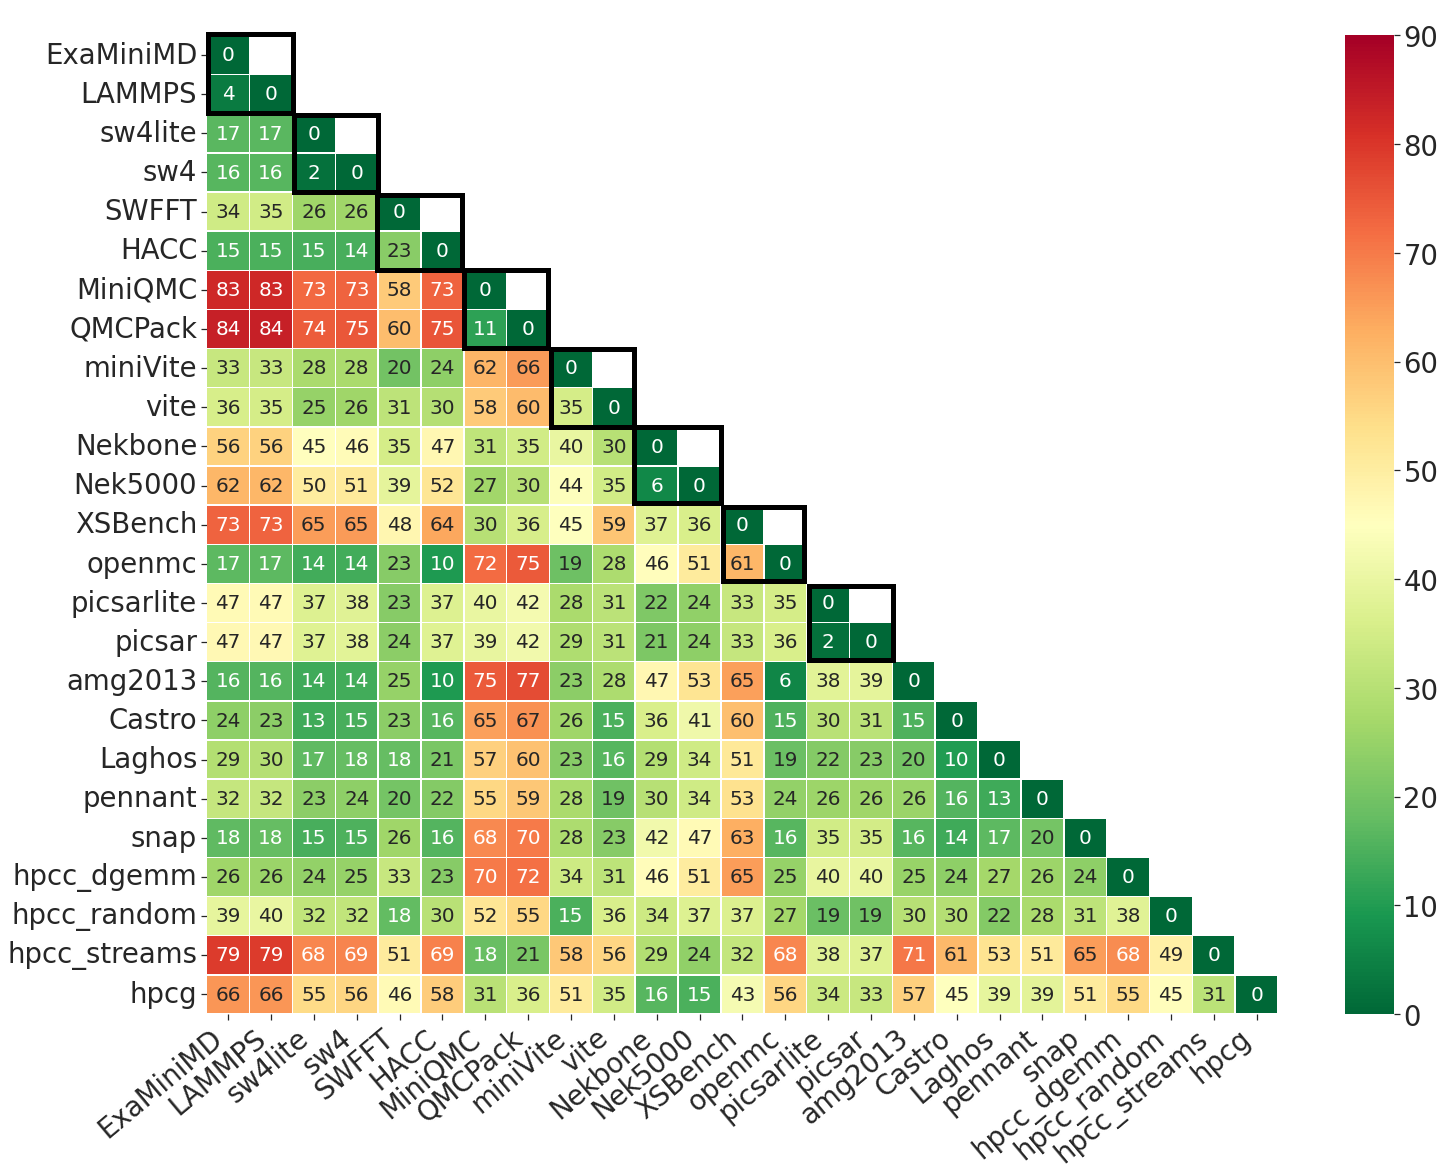
\includegraphics[width=3in]{figs/Cosine_origin_color_tri20.png}
	\vspace*{-5mm}
	\caption{Cosine Similarity}
	\label{figs:Cosine}
	\end{minipage}
\hspace{.1in}
\begin{minipage}[t]{0.48\textwidth}
	\centering
	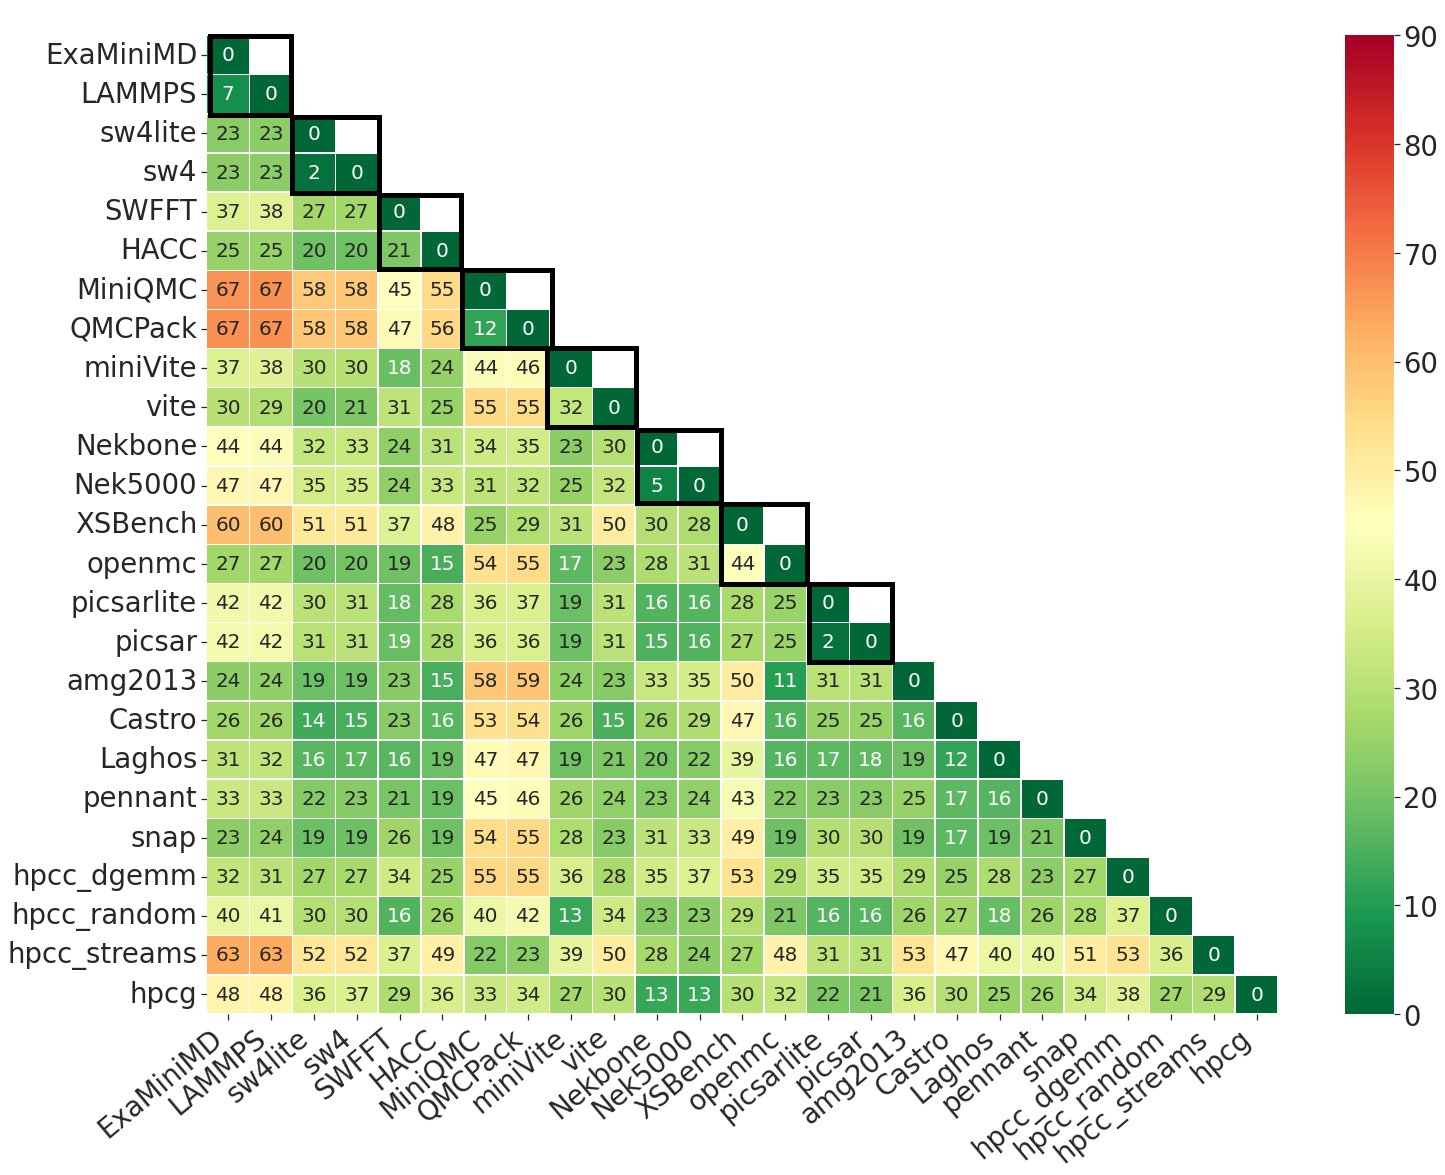
\includegraphics[width=3in]{figs/JS-divergence_m100.png}
	\vspace*{-5mm}
	\caption{JS divergence (Values are multiplied by 100)}
	\label{figs:JS}
	\end{minipage}
\hspace{.1in}
\begin{minipage}[t]{0.48\textwidth}
	\centering
	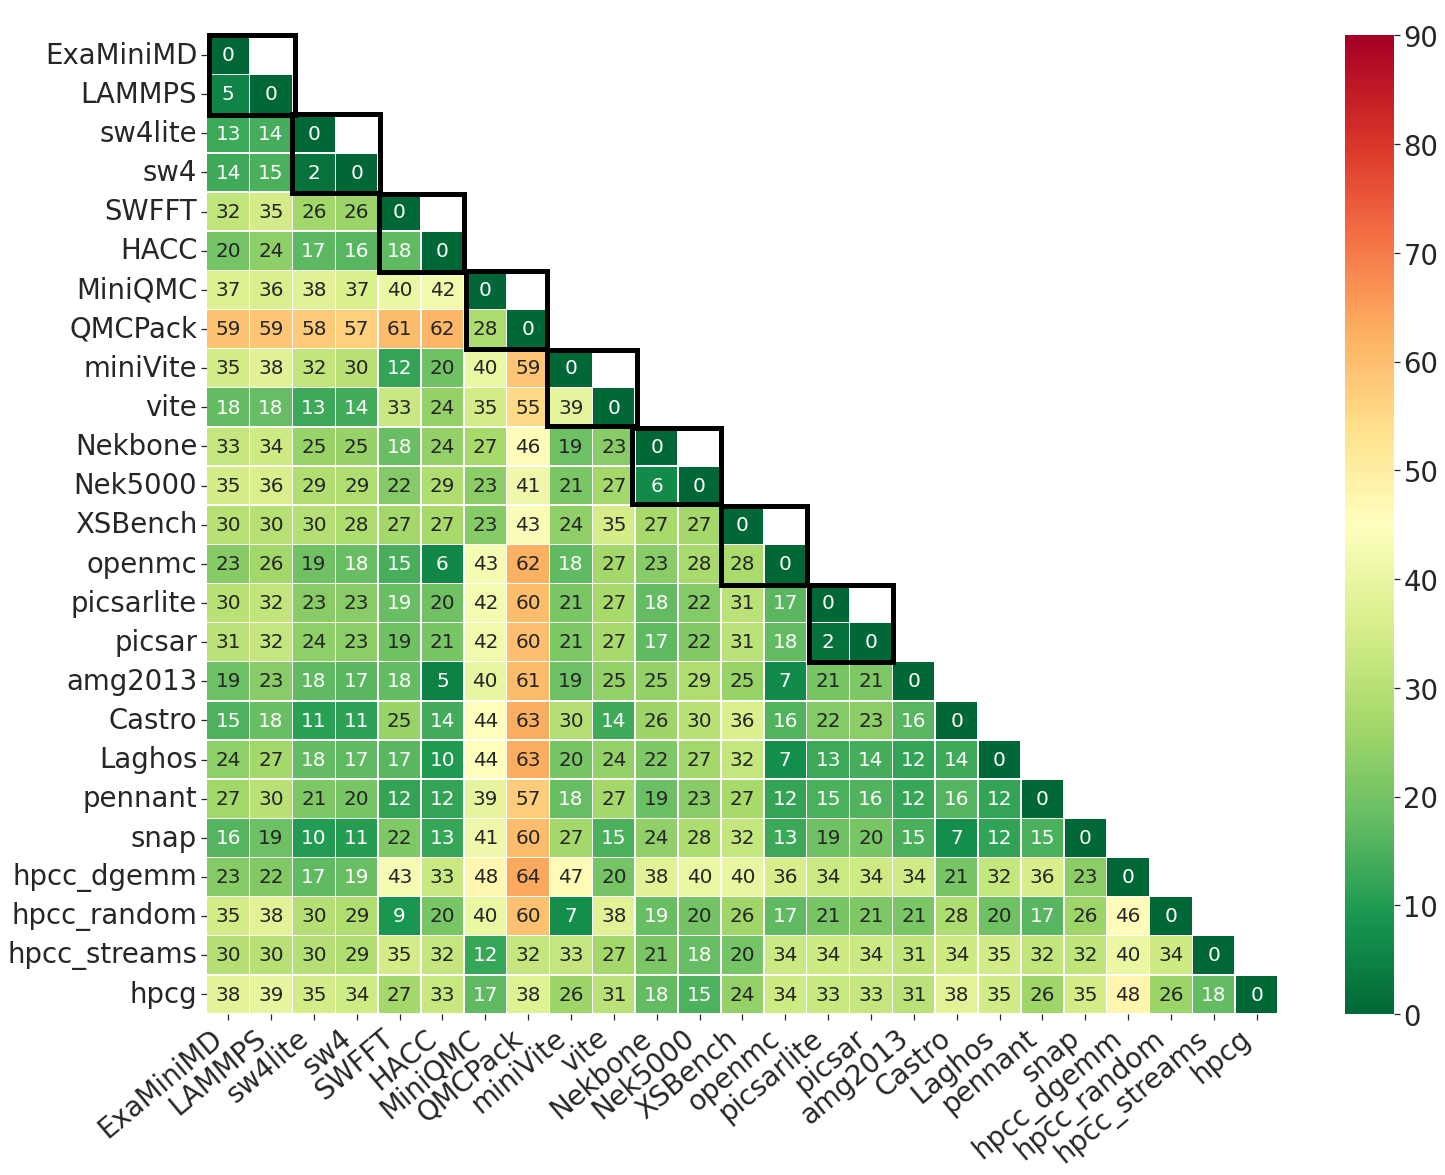
\includegraphics[width=3in]{figs/Wasserstein distance_m1000.png}
	\vspace*{-5mm}
	\caption{Wasserstein distance (Values are multiplied by 1000)}
	\label{figs:Wasserstein}
	\end{minipage}
\hspace{.1in}	
\begin{minipage}[t]{0.48\textwidth}
	\centering
	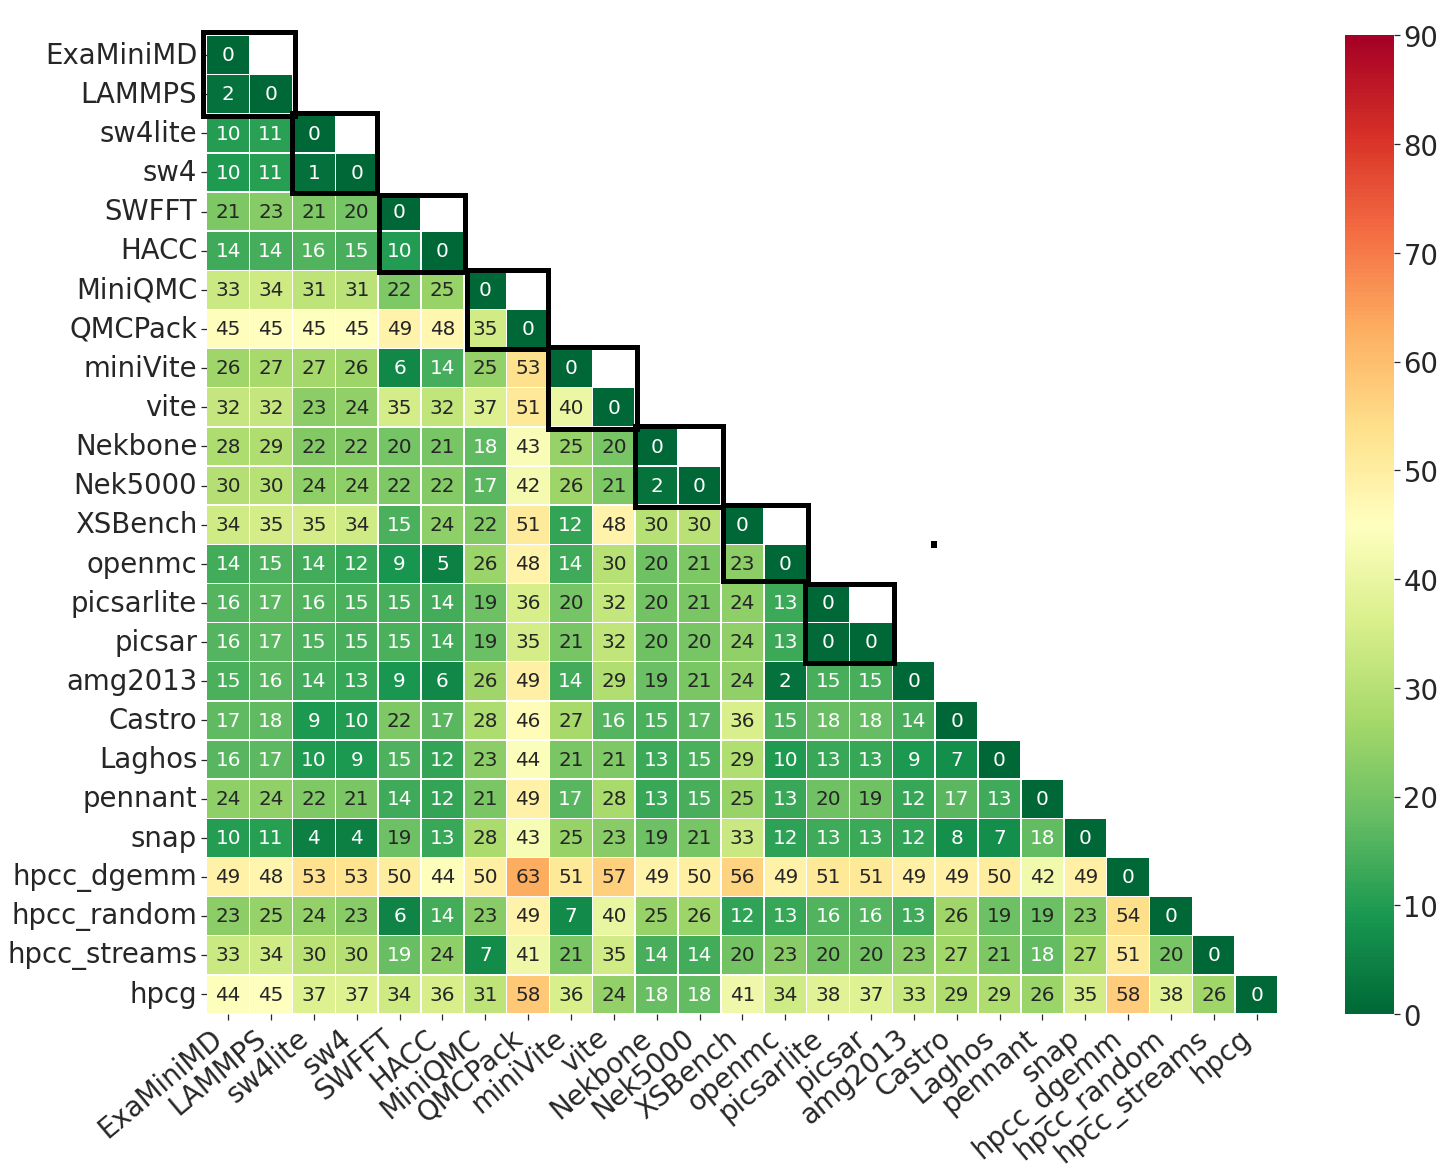
\includegraphics[width=3in]{figs/Mahalanobis distance_m10.png}
	\vspace*{-5mm}
	\caption{Mahalanobis distance (Values are multiplied by 10)}
	\label{figs:Mahalanobis}
	\end{minipage}
\hspace{.1in}
\end{figure*}

Since the similarity matrix is symmetric on the diagonal, we use the lower triangular heatmap to visualize the similarity. The diagonal entries are zero because they indicate the distances between the applications and themselves. We adjust the scale of value in each figure to be in the same range to make them comparable. The spectrum of colors that represent similarity is from a standard colormap, where dark green is highly similar and dark red is highly dissimilar. All proxies that have parents are listed first on the axes (top on y; left on x) and each parent is listed directly after its corresponding proxy. Along the diagonal, eight 2$\times$2 black border blocks circle the relationship between proxy and parent application pairs. One would expect to see the lower left of these blocks to be dark green, which shows a high similarity between proxy and parent. The nine miscellaneous applications (either a proxy with no parent or a parent with no proxy) are listed at the bottom on the y-axis and the right on the x-axis. 

Figures~\ref{figs:Cosine},~\ref{figs:JS},~\ref{figs:Wasserstein}, and~\ref{figs:Mahalanobis} are the overall feature results of four distance methods discussed in Section~\ref{sec:Sim} in the Skylake system. We can see that, generally, the four distance metrics we evaluate return similar correlations. Take for example Figure~\ref{figs:Cosine} which uses cosine similarity, PICSARlite and PICSAR, SW4lite and SW4, Nek5000 and Nekbone, ExaMiniMD and LAMMPS are highly similar proxy/parent application pairs. QMCPack and MiniQMC, and SWFFT and HACC show good similarity.  We get the \textbf{Observation 2}: \textit{75\% of the proxies in our suite demonstrate highly convergent behavior concerning their parents, and therefore, are faithful representations.} The other two pairs show some behavior gaps. miniVite and Vite are moderately similar. XSBench and OpenMC are highly dissimilar, with an angle of $60^\circ$ between them. This is probably because of the difference in complexity between the parent and proxy in this case; XSBench is only the cross-section lookup portion in Monte Carlo neutron transport, which is a highly data-intensive kernel, whereas OpenMC implements the full neutron transport code so likely has more opportunity to hide poor cache/memory behavior with other computation. The unpaired proxy applications (amg2013, Castro, Laghos, pennant, and snap) used as controls show relative similarity to each other, but do not match the known pairs. The other four HPC benchmark related applications are not similar to each other because they aim to measure totally different memory or data patterns. Another thing to note from Figure~\ref{figs:Cosine} is that application pairs QMCPack and MiniQMC are similar to one another but very different from other applications given lots of red and yellow colors. XSBench, Nekbone, Nek5000, PICSARlite, PICSAR, hpcc\_streams, and hpcg are also outliers in that their behavior shows significant differences compared to most other applications.  It's not surprising that hpcc\_streams is different from other applications because it's a synthetic benchmark program that measures sustainable memory bandwidth and the corresponding computation rate for a simple vector kernel. HPCG is designed to exercise computational and data access patterns that more closely match a different and broad set of important applications. In our suite, only Nekbone and Nek5000 are similar to hpcg.\si{?}

We also notice that there is some diversity when applying these four similarity algorithms. When looking at the dark red areas, applications hpcc\_streams and hpcg are highly dissimilar to other applications in cosine similarity, JS divergence, and Mahalanobis distance, while not that dissimilar in Wasserstein distance. This may be due to Wasserstein distance being impacted by the feature order in the vector. If the events that have divergent behavior locate far away in the vectors, the Wasserstein distance becomes bigger. The application hpcc\_degemm is extremely different from other applications in Mahalanobis distance but shows no obvious difference in other similarity algorithms. This may be because of the whitening process in Mahalanobis distance. QMCPack and MiniQMC diverge more in Wasserstein distance and Mahalanobis distance compared to the other two methods, and the difference mainly comes from the memory and cache subgroup which we will discuss in Sec~\ref{sec:subgroup}. It appears based on ~\cite{qmcpack} that much refactoring effort has gone into QMCPack to improve its memory
behavior and accuracy, and which has not been implemented in miniQMC. In conclusion, due to the principle of different similarity algorithms, the diversity of dissimilarity shows different ranges in four distance methods. Thus, we get the \textbf{Observation 3}: \textit{Similar proxy/parents application pairs remain similar no matter what similarity algorithm is used, while dissimilarities are not the same depending on what algorithm is used.}

Since these distance methods show similar results for similar pairs and the run-time difference of each method is negligible, cosine similarity becomes the preferred similarity metric for our problem due to its simplicity, performance, and ease of interpretability by geometric angle.

\subsection{Important features}
% Laplacian score method requires more sample points for accuracy. Therefore, besides the averaged accumulated data, we also include the original 5 trials' accumulated data. 
Since we assume each application shows similar performance in different trials, and proxy and parent applications show similar performance, we set the parameter of neighbor size to be 2 in the Laplacian score algorithm. After removing the correlated features via the correlation filter, we get 89 ranked features. Table~\ref{tab:top20Cosine} lists the top 20 features, and Figure~\ref{figs:top20Cosine}  shows the cosine similarity matrix using these 20 features. Compared to using all the 500 features as in Figure~\ref{figs:Cosine}, using only the top 20 features can produce more easily graspable similarity information. As we can see in Figure~\ref{figs:top20Cosine}, all 2$\times$2 black border blocks that show high similarity between proxy and parent are preserved. Unsurprisingly, applications that are not pairs remain dissimilar.% the general trend while not the same as the original ones.

\begin{table*}[t]
\caption{Top 20 features}
\label{tab:top20Cosine}
\centering
\begin{tabular}{ll}
\toprule
\small
\textbf{Rank} & \multicolumn{1}{c}{\textbf{Hardware event count names}}            \\ \midrule
1             & `MEM\_LOAD\_UOPS\_L3\_HIT\_RETIRED:XSNP\_NONE'                     \\ 
2             & `OFFCORE\_REQUESTS:DEMAND\_DATA\_RD'                               \\ 
3             & `UOPS\_EXECUTED:THREAD'                                            \\ 
4             & `OFFCORE\_REQUESTS\_OUTSTANDING:ALL\_DATA\_RD'                     \\ 
5             & `OFFCORE\_REQUESTS\_BUFFER:SQ\_FULL'                               \\ 
6             & `MEM\_LOAD\_UOPS\_L3\_MISS\_RETIRED:LOCAL\_DRAM'                   \\ 
7             & `MEM\_LOAD\_UOPS\_RETIRED:HIT\_LFB'                                \\ 
8             & `CYCLE\_ACTIVITY:CYCLES\_L1D\_MISS'                                \\ 
9             & `OFFCORE\_REQUESTS\_OUTSTANDING:ALL\_DATA\_RD\_CYCLES'             \\ 
10            & `CYCLE\_ACTIVITY:CYCLES\_LDM\_PENDING'                             \\ 
11            & `EXE\_ACTIVITY:3\_PORTS\_UTIL'                                     \\ 
12            & `OFFCORE\_REQUESTS\_OUTSTANDING:L3\_MISS\_DEMAND\_DATA\_RD'        \\ 
13            & `BR\_INST\_RETIRED:NEAR\_CALL'                                     \\ 
14            & `OFFCORE\_REQUESTS:ALL\_REQUESTS'                                  \\ 
15            & `ARITH:DIVIDER\_ACTIVE'                                            \\ 
16            & `ICACHE\_64B:IFTAG\_HIT'                                           \\ 
17            & `MEM\_UOPS\_RETIRED:STLB\_MISS\_LOADS'                            \\ 
18            & `OFFCORE\_REQUESTS\_OUTSTANDING:L3\_MISS\_DEMAND\_DATA\_RD\_GE\_6' \\ 
19            & `UOPS\_DISPATCHED:PORT\_1'                                         \\ 
20            & `MEM\_UOPS\_RETIRED:SPLIT\_STORES'                                 \\ \bottomrule
\end{tabular}
\normalsize
\end{table*}

\begin{figure}[ht]
\centering
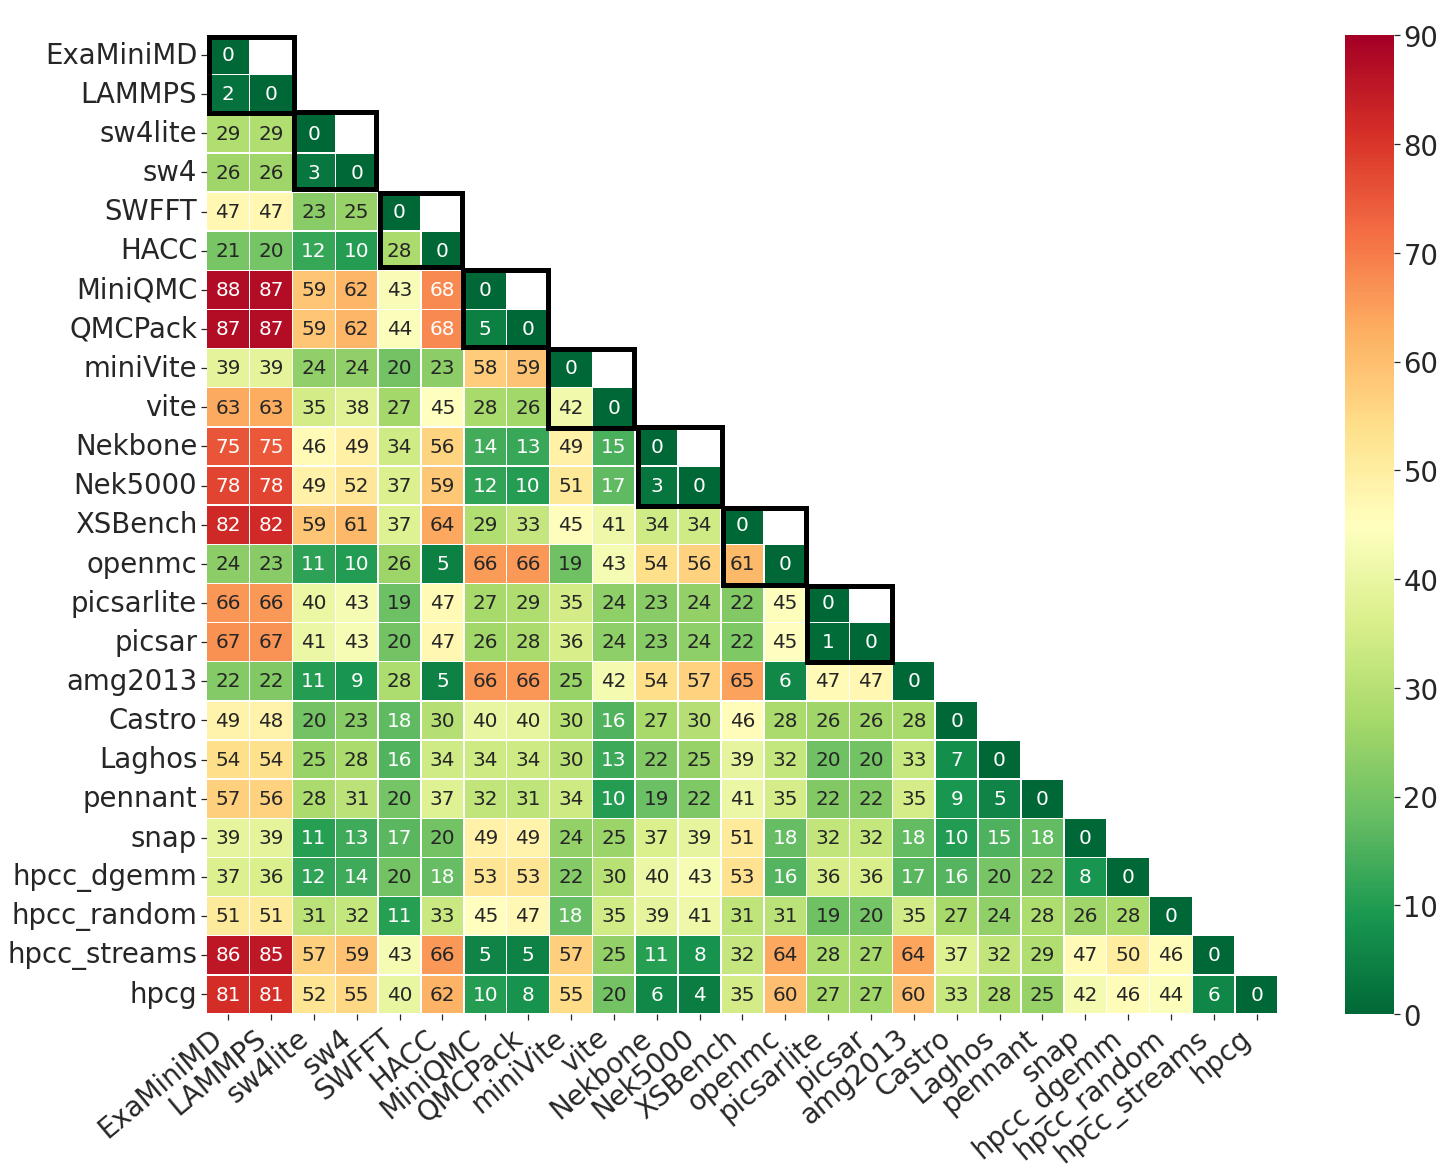
\includegraphics[width=\linewidth]{figs/top20cosine_origin_color_font20.png}
\caption{Cosine Similarity with top 20 important features}
\label{figs:top20Cosine}
\end{figure}

\subsection{Feature Standard Deviation}
\label{sec:Dev}
Besides selecting the important features to preserve the similarity of proxy and parent pairs, we are also curious about what contributes to the dissimilarity of the proxy and parent pairs. Therefore, we investigate the run-time time series. Using the data of hardware event counts per second, we get the standard deviation for each application on each feature (hardware event counts). If one point is located within 2 standard deviations, we consider this point to be within the distribution.


We calculate the standard deviation of each feature for each parent application and check whether the accumulated mean of the according feature of a proxy application is within two standard deviations of the parents' accumulated mean within a normal distribution. 
Table~\ref{tab:Dissimilarity} shows the feature numbers for each proxy/parent pair when the difference is bigger than 2, 3, 4, 5 standard deviations separately. The result is as we expected as in Figure~\ref{figs:Cosine}. We can see that SW4lite and SW4, and PISCARlite and PISCAR, are the most similar proxy/parent pairs because, in each pair, the proxy only has one feature (`MOVE\_ELIMINATION: SIMD\_NOT\_ELIMINATED' and `UOPS\_EXECUTED: X87' separately) deviate relatively far from the parent. The proxies that have more features deviating farther from their parents are accordingly less similar. \eg miniVite and Vite have 72 features with large deviation, and they are moderately similar with 35 degrees in the cosine similarity matrix Figure~\ref{figs:Cosine}. This 
brings us \textbf{Observation 4}: \textit{A proxy application that has most of the hardware event counts within standard deviations of the parent application is similar to its parent.} 



\begin{table}[t]
\caption{Dissimilarity feature source for proxy/parents pairs}
\label{tab:Dissimilarity}
\centering
\begin{tabular}{lrrrr}%llll}
\toprule
\textbf{Proxy and Parent pairs}               & \textbf{\textgreater{}2std} & \textbf{\textgreater{}3std} & \textbf{\textgreater{}4std} & \textbf{\textgreater{}5std} \\ \midrule
ExaMiniMD / LAMMPS                            & 10                          & 8                           & 8                           & 4                           \\ 
SW4lite / SW4                                 & 1                           & 1                           & 1                           & 1                           \\ 
SWFFT / HACC                                  & 17                          & 12                          & 11                          & 8                           \\ 
miniQMC / QMCPACK                             & 13                          & 10                          & 8                           & 6                           \\ 
miniVite / Vite                               & 72                          & 38                          & 23                          & 21                          \\ 
Nekbone / Nek5000                             & 11                          & 6                           & 2                           & 2                           \\ 
XSbench OpenMC                                & 16                          & 9                           & 9                           & 8                           \\ 
PICSARlite / PICSAR                           & 1                           & 1                           & 1                           & 0                           \\ 
Unique feature \#s & 99                          & 64                          & 49                          & 38                          \\ \bottomrule
\end{tabular}

\end{table}


\subsection{Subgroup Features}
\label{sec:subgroup}
In addition to studying the features overall, we also investigate the similarity in subgroups, since we collect the data in subgroups as in Sec \ref{sec:collect}. We could focus on a subgroup behavior that we are interested in, instead of considering them overall. 
For example, if one is using this data to choose proxy applications for a memory study, memory behavior diversity can have a much larger impact on the choice. In contrast, if one is using this data to decide if a proxy can be used to examine refactoring code for improved memory performance, a small difference between proxy and parent in memory may not matter. 

We look at many subgroups of data. Some subgroup (\eg, Branch, Instruction Mix, Instruction Cache, and L3 Cache) matrices have no colors other than green or light green (no dissimilarity), while others show the applications which are outliers in those subgroups. Here we show some matrices that have extensive dissimilarities. Figure~\ref{figs:cosine L1_D_Cache} shows similarity over only L1 cache related performance counters. We can see that applications MiniQMC and QMAPack are relatively
similar to each other but dissimilar to others in this subgroup. In the memory pipeline subgroup (Figure~\ref{figs:cosine Memory_Pipeline}), ExaMiniMD and LAMMPS show dissimilarity to others. In the Execution Pipeline subgroup (Figure~\ref{figs:cosine Execution_Pipeline}), MiniQMC, QMAPack, XSBench, hpcc\_streams have divergent behavior from all other applications. Thus, we get the \textbf{Observation 5}: \textit{Outliers are not consistent in different subgroups.}
We cannot describe all examples in this paper, but the investigation of subgroups gives us a way to see similarities in specific fields.%\avani{can we add this to an appendix?} \si{appendix counts in pages}

\begin{figure}[ht]
\centering
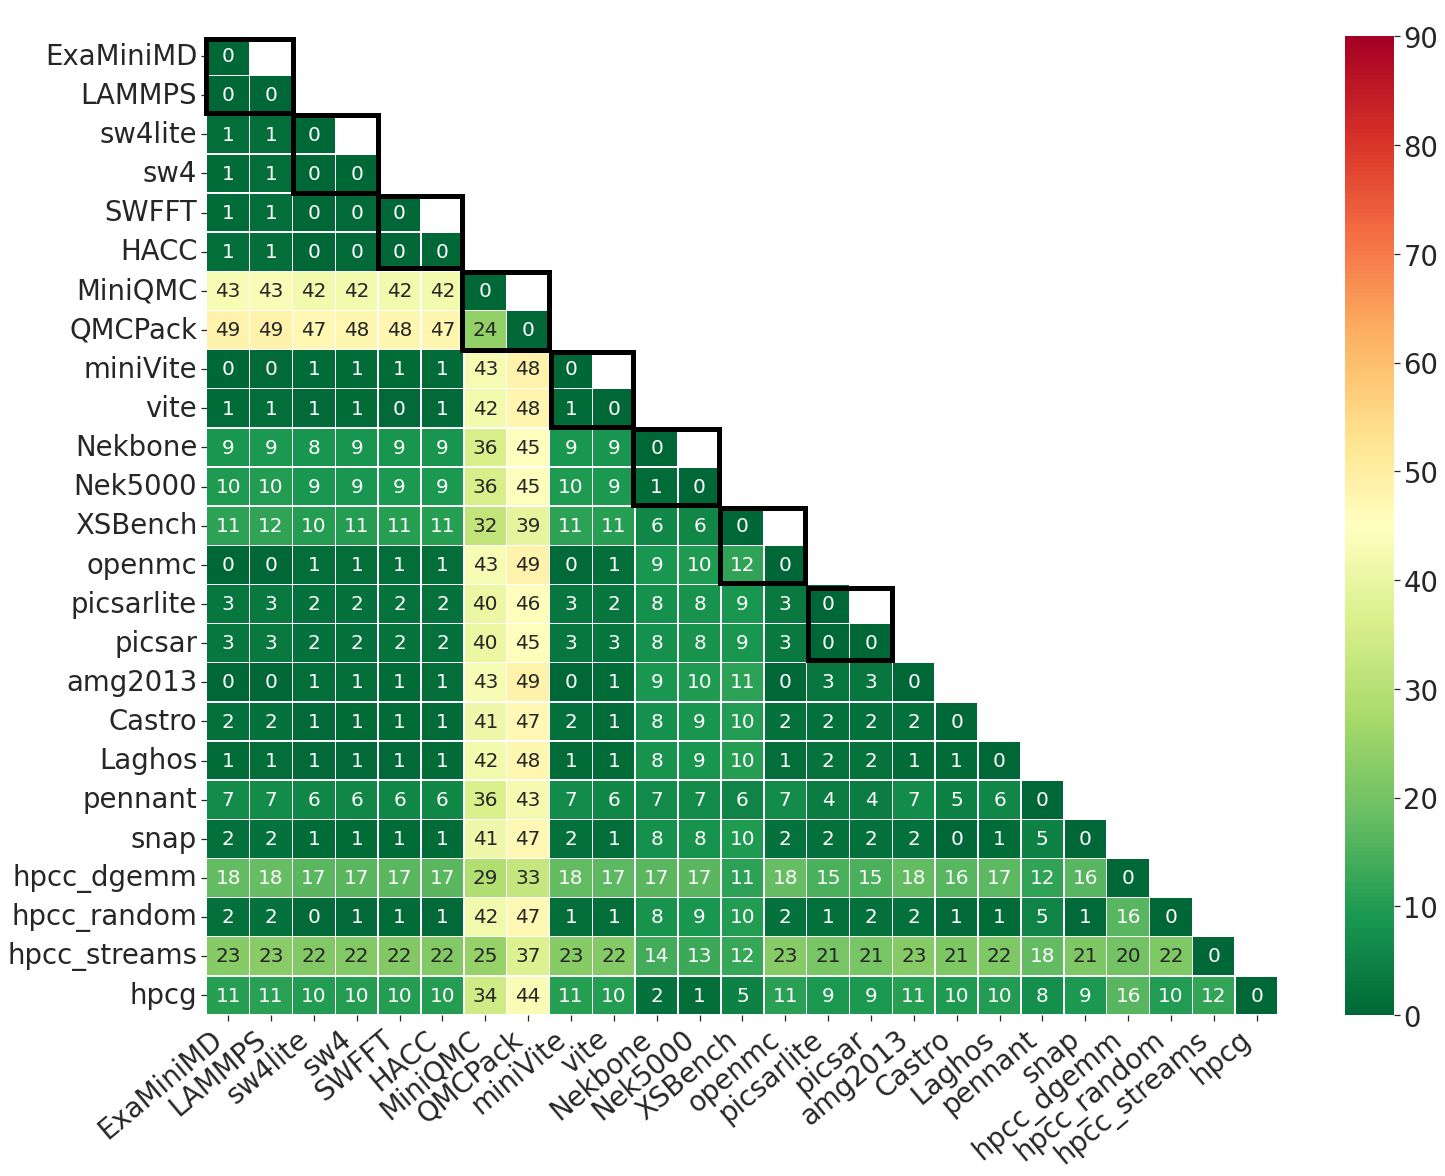
\includegraphics[width=0.9\linewidth]{figs/L1_Cache_font20.png}
\caption{Cosine Similarity for L1 Cache }
\label{figs:cosine L1_D_Cache}
\end{figure}

\begin{figure}[ht]
\centering
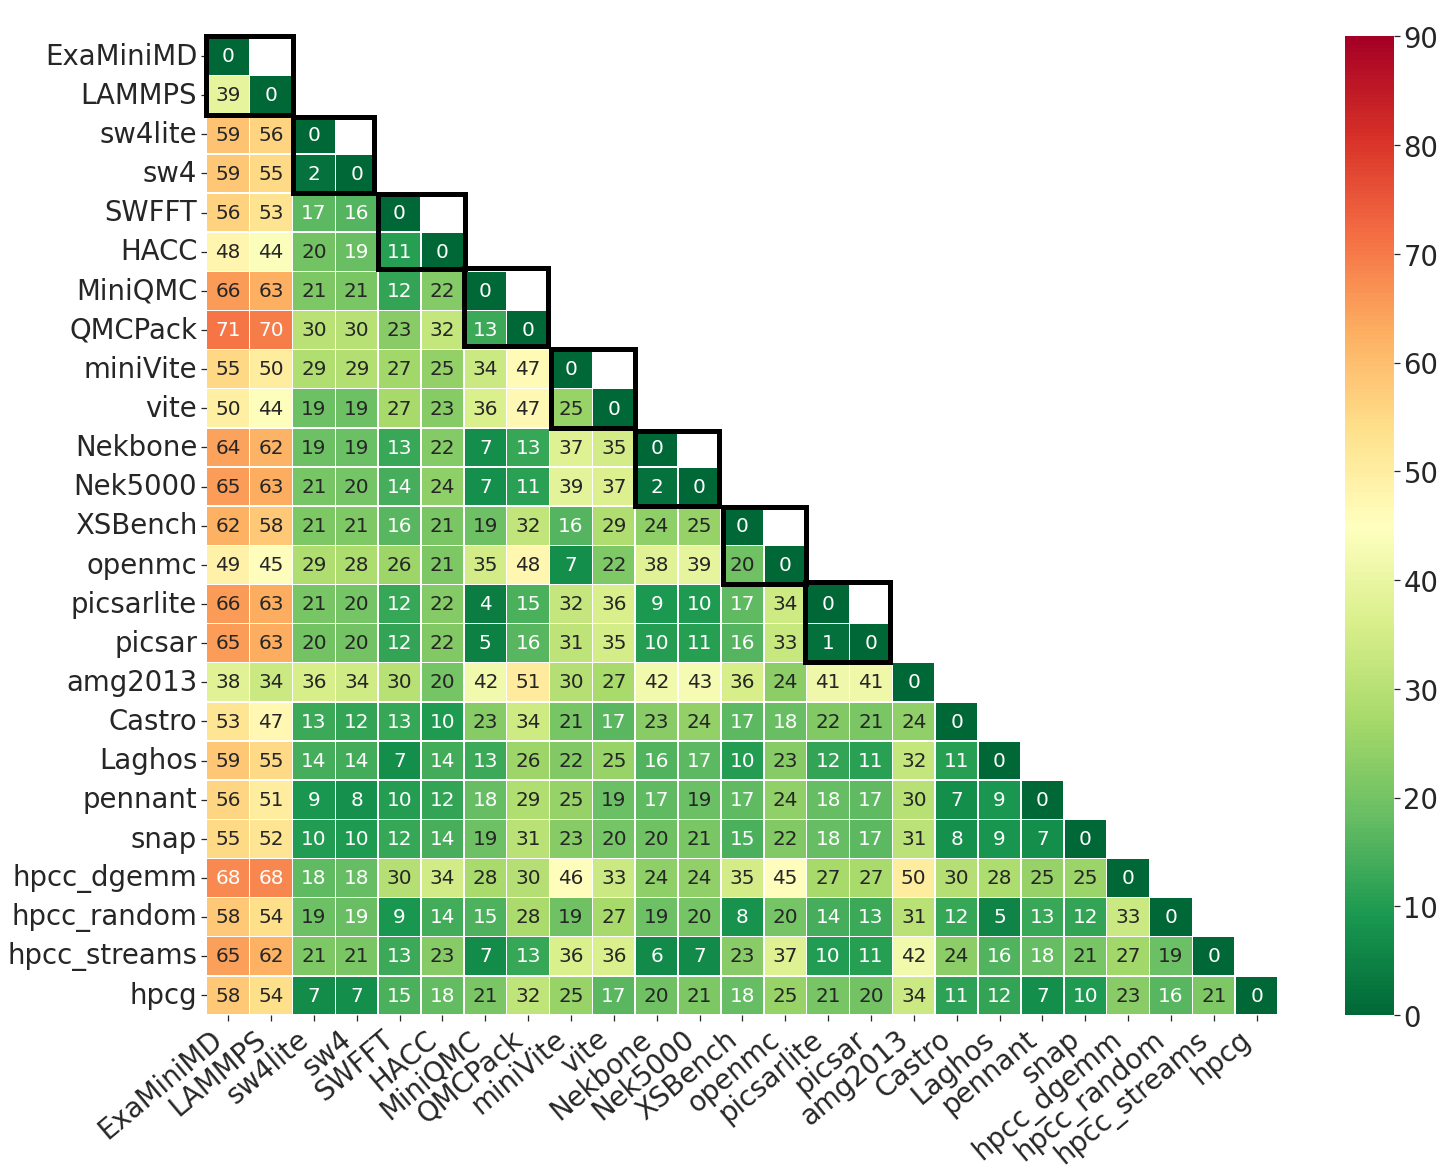
\includegraphics[width=0.9\linewidth]{figs/Memory_Pipeline.png}
\caption{Cosine Similarity for Memory Pipeline }
\label{figs:cosine Memory_Pipeline}
\end{figure}

\begin{figure}[ht]
\centering
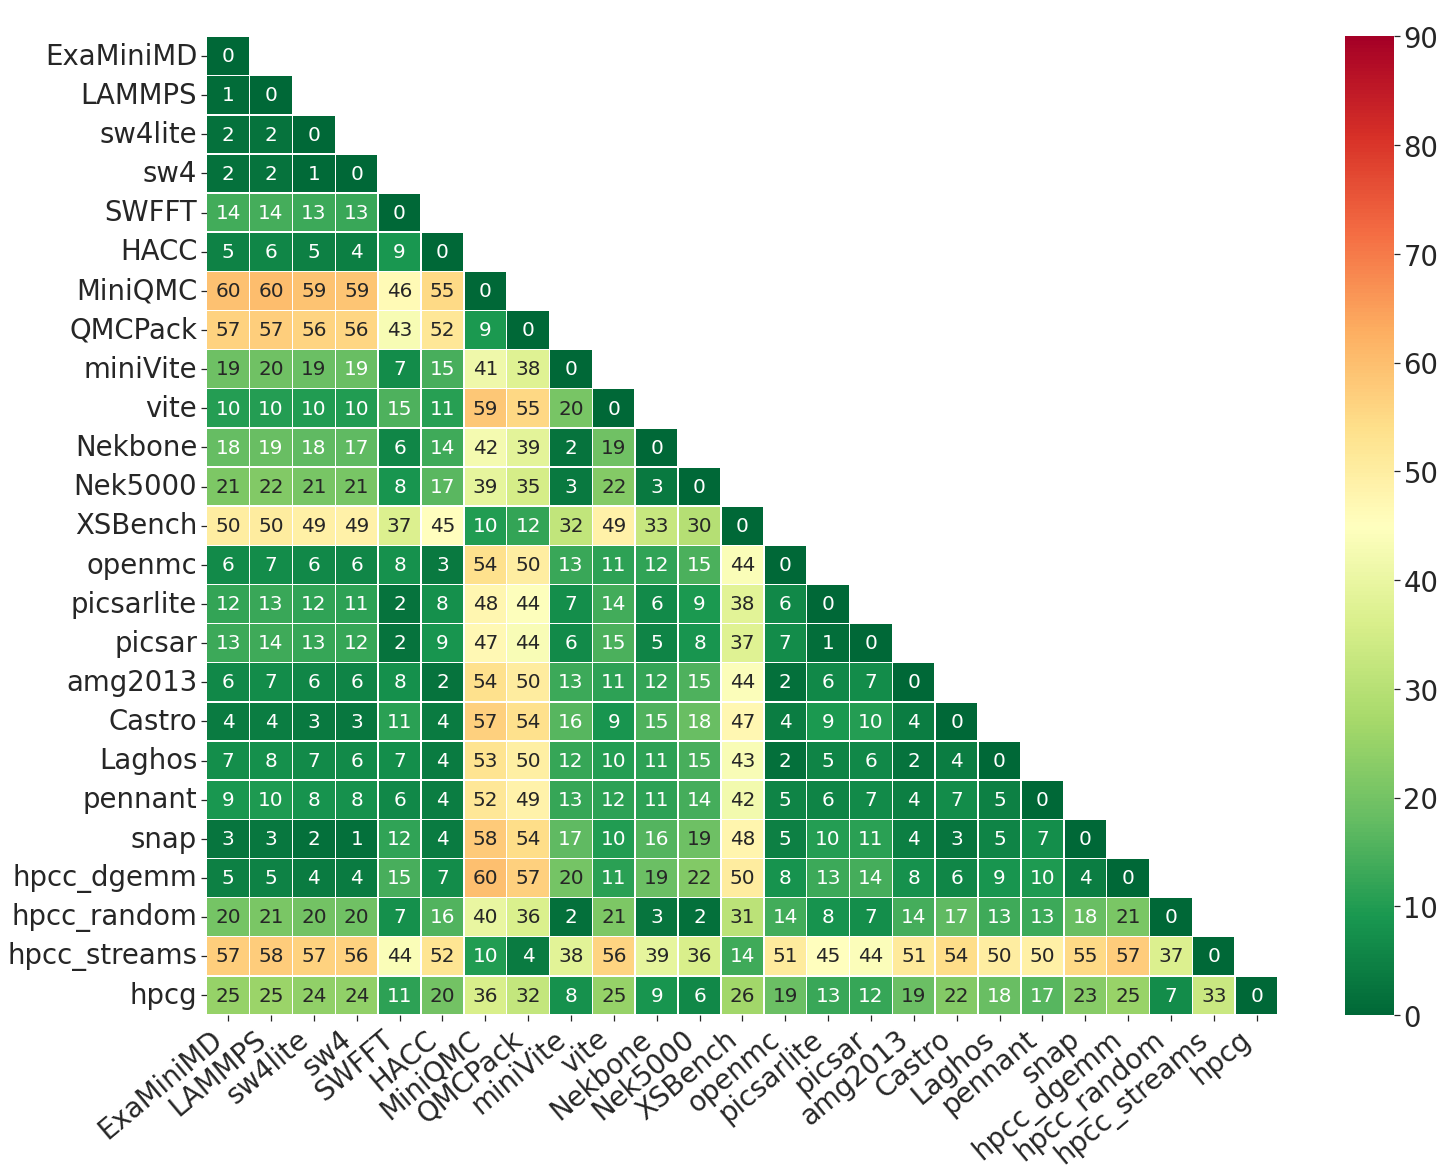
\includegraphics[width=0.9\linewidth]{figs/Execution_Pipeline.png}
\caption{Cosine Similarity for Execution Pipeline }
\label{figs:cosine Execution_Pipeline}
\end{figure}


\subsection{Discussion}
\avani{to expand}
%\si{shall we move this to discussion?}
%Notice that to collect the complete set of data, we run each application multiple times. Run-time variance is inevitable among multiple runs. Therefore, when we combine all the features if we want to keep the time phases, we need to consider aligned data. The run-time differences also occur among different applications, \eg most parent applications have longer run-time than corresponding proxy applications. Since our current analysis is based on the final accumulated average of each hardware event counts for each application, we temporarily do not take the run-time differences into account. For future work of time phases comparison, we have implemented run-time alignment for each application with a weighted index for each run. 
Our results indicate, surprisingly, that the particularities of the similarity algorithms have less impact than predicted on the likelihood of correlating parent/proxy pairs.  Since we use ECP pairs, we expect that this is a general result, but we cannot rule out the possibility that some domains will not have clearly separable parent/proxy relationships.

Run-time variance is inevitable in HPC. On the one hand, to collect the complete set of data, we run each application multiple times. Minor run-time differences occur among multiple runs. On the other hand, different applications vary in run-time, \eg most parent applications have longer run-time than their corresponding proxy applications. Since our current analysis is based on the final accumulated average of each hardware event count for each application, we temporarily do not take these run-time differences into account. However, if we want to keep the time phases for each application, we need to consider aligned data. Currently, we have implemented run-time alignment for each application with a weighted index for each run, but aligned data could be used for future time phase comparison. 

For future work, we will evaluate the important features on more platforms. Since currently our analysis is based on the final accumulated average of each hardware event counts, the variance of run time for each application is negligible after we average the results. Therefore, we do not take time phases into account. Recently, We have implemented run-time alignment for each application. For the next step, we will analyze the time phases across proxy/parent application pairs.

\todo{List / expand upon other places this could be used: compiler studies, to understand what's different when refactoring applications}  \jeanine{todo}